\chapter{Methods}


\section{Design}
%-------------------------------------------%

\begin{figure}
	\caption{"Data flow within our software stack"}
	\centering
		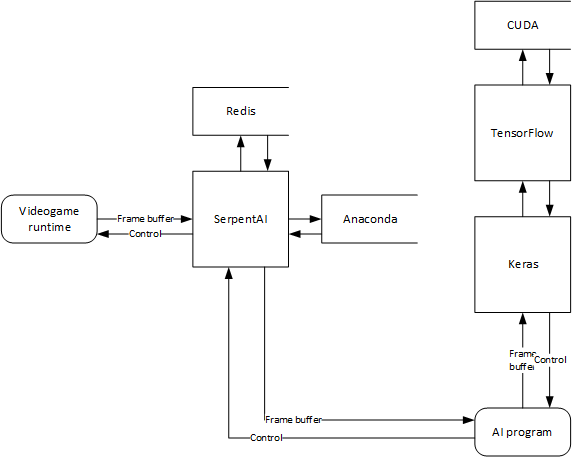
\includegraphics[scale = 0.75]{dataflow.png} \\
\end{figure}

%-------------------------------------------%


\section{Frameworks}
%-------------------------------------------%

Our project uses a software stack comprised of the following modules and libraries: {\it SerpentAI}, {\it Keras}, {\it TensorFlow}, and the {\it Anaconda Distribution} for Python 3.

We chose to use Python 3 as our primary programming language for its flexibility, intuitive syntax, and data processing capabilities. Python is also helpfully compatible with all of the other software listed above. Furthermore, the {\it Anaconda distribution} provides us with a large assortment of Python modules, some of which {\it SerpentAI} cites as dependencies \cite{SerpentAI}. This allows us to more easily work from within a Windows environment, which in turn gives us the most straightforward and stable access to GPU computation via NVIDIA proprietary drivers.

{\it SerpentAI} is an open source Python framework that allows researchers to write scripts that can easily retrieve the frame buffer from a game and then send keyboard or controller input back to it. The framework is noteworthy for functioning entirely independently of the target game. Furthermore, it makes no presumptions about what machine learning techniques the user wants to implement and can support anything from simple reflex or random agents to the most advanced and cutting-edge neural networks \cite{SerpentAI}. Ergo, {\it SerpentAI} serves as a bridge between our artificial intelligence and its testing environment by providing a simple interface for retrieving frame buffer data from and sending control input to virtually any game runtime. This is achieved by writing a game agent program. Our game agent utilizes {\it TensorFlow}, which is self-described as ``an open source software library for numerical computation using data flow graphs,'' was designed explicitly for use in machine learning research, and is able to achieve exceptional performance by employing either GPU computation or SIMD CPU instruction set architectures, such as SSE \cite{TensorFlow}. However, our agent does not access {\it TensorFlow} directly. Rather, it uses {\it Keras}, a high-level machine-learning library designed to serve as an abstraction layer over foundational libraries like {\it TensorFlow}. The low-level library still performs all of the heavy-lifting; {\it Keras} simply removes some of the barriers to entry \cite{Keras}.

The target game for this project is {\it Rivals of Aether}, a 2D fighting game created by independent game developer Dan Fornace \cite{RivalsofAether}. We selected {\it Rivals of Aether} because it supports the recording of replays, which are files that keep a record of what controller inputs were detected from which player during each frame of gameplay. Thus, whereas a conventional video recording associates each frame with its pixel data, a replay does so with each frame and its input data. This allows the game to simulate a past match in real-time with perfect accuracy by simply running a new match in which each player's control input is read from the replay file rather than from the controller.

\begin{figure}
	\caption{"Screenshot showing gameplay in Rivals of Aether"}
	\centering
	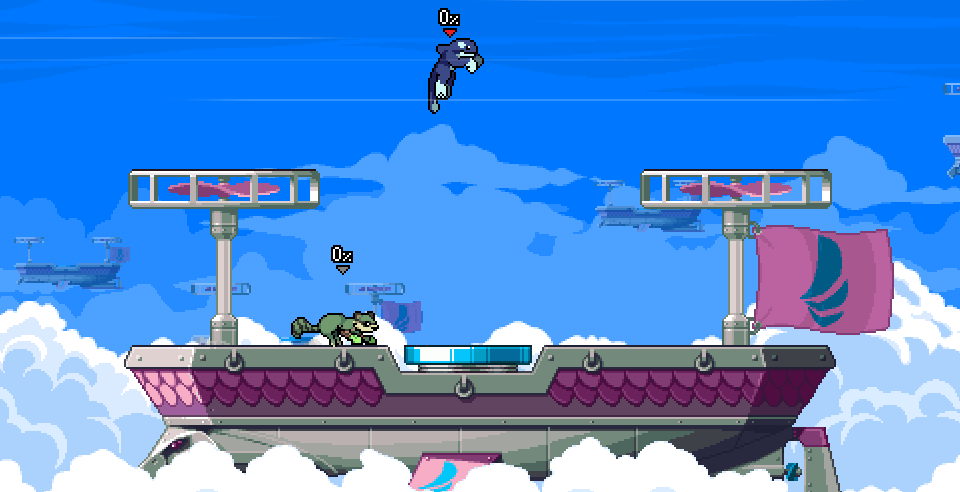
\includegraphics[scale = 0.5]{game.png} \\
\end{figure}

A replay file is therefore no different from a demo file from {\it Quake} or {\it Doom}. Such demos are often used in game-related machine learning research because a collection of demos is effectively a pre-labeled dataset. However, unlike {\it Doom} and {\it Quake}, which have websites such as {\it Speed Demo Archives} and {\it Quake Terminus}, {\it Rivals of Aether} does not have any well-established public repositories for replay files. Therefore, in order to build our collection of replays, we solicited from the {\it Rivals of Aether} community. Contributors provided us with a total of 1,020 replay files from a variety of settings, including tournaments, exhibitions, ranked matches, and private games. Adding our own personal replays brings the total up to 1,032. 

We have opted to use our own personal computers running 64-bit Windows 10 with Ubuntu subsystems as both our platform and development environment. There are several reasons to justify this decision. Firstly, we wanted to ensure that we would have the best possible experience when dealing with GPU computation, and NVIDIA simply has a longer and better track record for supporting Windows than it does for Linux. Secondly, we wanted to avoid the potential pitfall of our platform restricting us to a smaller library of target games. Our two top candidates were {\it Quake} and {\it Rivals of Aether} because both of these games support replays, or demos; however, of those two games, only {\it Quake} natively supports Linux, and ultimately we selected {\it Rivals of Aether}. Lastly, and with regards to using our own computers for both development and testing, we made the decision to abstain from distributed or cloud computing chiefly to save costs, but also as an aesthetic choice based in the desire to see what our computers are capable of. Despite all of the above justifications for using Windows, it remains to be said that our project cannot live without Linux. {\it SerpentAI} requires a Redis database, so in order for that to work we use an Ubuntu subsystem; this is the official recommendation from the {\it SerpentAI} developers \cite{SerpentAI}.

%-------------------------------------------%



\section{Algorithms}
%-------------------------------------------%

Descriptions and pseudocode of important algorithms in use, relevant, or to be implemented as part of your project.

%-------------------------------------------%



\section{Analytical Methods}
%-------------------------------------------%

Descriptions and processes of any analytical methods used as part of your capstone project. This section is most applicable for projects with a data analysis focus or component. Quantitative and qualitative methods.

%-------------------------------------------%



\section{Features}
%-------------------------------------------%

A brief overview of primary features you plan to implement.

\begin{figure}
	\caption{"Keyboard controls for Rivals of Aether"}
	\centering
	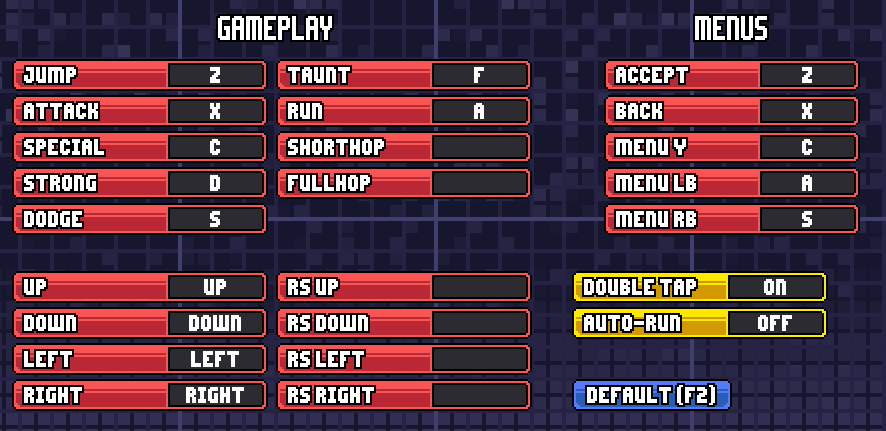
\includegraphics[scale = 0.75]{controls.png} \\
\end{figure}

%-------------------------------------------%



\section{Test Plan}
%-------------------------------------------%

We have over 1,000 data points in the form of replay files. This dataset will be randomly distributed such that around eighty-percent goes into a training set, fifteen-percent into a testing set, and the remainder into a validation set.

A training session will run as follows. The {\it SerpentAI} agent will traverse the game's menus to initiate playback of the next replay from a shuffled copy of the training set. While the match is simulated, the agent will simultaneously read the visual buffer from the game and control input data from the replay file. For each frame, the agent will pair the input data with its corresponding visual buffer and then send this bundle to a {\it TensorFlow} neural network as labels and data, respectively. The neural network will attempt to produce a set of appropriate control inputs in response and adjust its weights  whenever its prediction are incorrect. When playback has concluded, the agent will traverse the menus once again to start a new replay, repeatedly, until it has reached its quota. The total number of training iterations will vary between experiments until it produces satisfactory results.

A properly trained neural network shall demonstrate several qualities other than a high accuracy when tested against the held back data. Firstly, it shall be able to defeat low-level in-game bots, thereby demonstrating its competence. This can be tested by placing the neural network in matches against bots of increasing difficulty, thereby enabling the assignment of numerical performance benchmarks. Secondly, it shall play in a believably-human manner. This means that it should, wherever possible, be discouraged from playing {\it inhumanly} well, getting stuck, or displaying mechanical tics. Examples of these undesirable behaviors would include, in order, executing nonstop frame-perfect moves throughout the course of an entire game, running off of the stage or standing still due to an as-of-yet unseen situation, or constantly changing direction for no reason while otherwise playing competently. Identifying all such behaviors will be difficult prior to live experiments, however.

%-------------------------------------------%



\section{Criteria and Constraints}
%-------------------------------------------%

Project development must meet desired needs within realistic constraints. Many times, constraints are interrelated. Cover the appropriate criteria and constraints related to your capstone. Some example criteria and constraints are health and safety, environmental, political, social, manufacturability, sustainability, economical, and ethical.

%-------------------------------------------%